%%%%%%%%%%%%%%%%%%%%%%%%%%%%%%%%%%%%%%%%%%%%%%%%%%%%%%%%%%%%%%%%%%%%%%
%%  Copyright by Wenliang Du.                                       %%
%%  This work is licensed under the Creative Commons                %%
%%  Attribution-NonCommercial-ShareAlike 4.0 International License. %%
%%  To view a copy of this license, visit                           %%
%%  http://creativecommons.org/licenses/by-nc-sa/4.0/.              %%
%%%%%%%%%%%%%%%%%%%%%%%%%%%%%%%%%%%%%%%%%%%%%%%%%%%%%%%%%%%%%%%%%%%%%%

\documentclass[11pt]{article}

\usepackage[most]{tcolorbox}
\usepackage{times}
\usepackage{epsf}
\usepackage{epsfig}
\usepackage{amsmath, alltt, amssymb, xspace}
\usepackage{wrapfig}
\usepackage{fancyhdr}
\usepackage{url}
\usepackage{verbatim}
\usepackage{fancyvrb}
\usepackage{adjustbox}
\usepackage{listings}
\usepackage{color}
\usepackage{subfigure}
\usepackage{cite}
\usepackage{sidecap}
\usepackage{pifont}
\usepackage{mdframed}
\usepackage{textcomp}
\usepackage{enumitem}


% Horizontal alignment
\topmargin      -0.50in  % distance to headers
\oddsidemargin  0.0in
\evensidemargin 0.0in
\textwidth      6.5in
\textheight     8.9in 

\newcommand{\todo}[1]{
\vspace{0.1in}
\fbox{\parbox{6in}{TODO: #1}}
\vspace{0.1in}
}


\newcommand{\unix}{{\tt Unix}\xspace}
\newcommand{\linux}{{\tt Linux}\xspace}
\newcommand{\minix}{{\tt Minix}\xspace}
\newcommand{\ubuntu}{{\tt Ubuntu}\xspace}
\newcommand{\setuid}{{\tt Set-UID}\xspace}
\newcommand{\openssl} {\texttt{openssl}}


\pagestyle{fancy}
\lhead{\bfseries SEED Labs}
\chead{}
\rhead{\small \thepage}
\lfoot{}
\cfoot{}
\rfoot{}


\definecolor{dkgreen}{rgb}{0,0.6,0}
\definecolor{gray}{rgb}{0.5,0.5,0.5}
\definecolor{mauve}{rgb}{0.58,0,0.82}
\definecolor{lightgray}{gray}{0.90}


\lstset{%
  frame=none,
  language=,
  backgroundcolor=\color{lightgray},
  aboveskip=3mm,
  belowskip=3mm,
  showstringspaces=false,
%  columns=flexible,
  basicstyle={\small\ttfamily},
  numbers=none,
  numberstyle=\tiny\color{gray},
  keywordstyle=\color{blue},
  commentstyle=\color{dkgreen},
  stringstyle=\color{mauve},
  breaklines=true,
  breakatwhitespace=true,
  tabsize=3,
  columns=fullflexible,
  keepspaces=true,
  escapeinside={(*@}{@*)}
}

\newcommand{\newnote}[1]{
\vspace{0.1in}
\noindent
\fbox{\parbox{1.0\textwidth}{\textbf{Note:} #1}}
%\vspace{0.1in}
}


%% Submission
\newcommand{\seedsubmission}{You need to submit a detailed lab report, with screenshots,
to describe what you have done and what you have observed.
You also need to provide explanation
to the observations that are interesting or surprising.
Please also list the important code snippets followed by
explanation. Simply attaching code without any explanation will not
receive credits.}

%% Book
\newcommand{\seedbook}{\textit{Computer \& Internet Security: A Hands-on Approach}, 2nd
Edition, by Wenliang Du. See details at \url{https://www.handsonsecurity.net}.}

%% Videos
\newcommand{\seedisvideo}{\textit{Internet Security: A Hands-on Approach},
by Wenliang Du. See details at \url{https://www.handsonsecurity.net/video.html}.}

\newcommand{\seedcsvideo}{\textit{Computer Security: A Hands-on Approach},
by Wenliang Du. See details at \url{https://www.handsonsecurity.net/video.html}.}

%% Lab Environment
\newcommand{\seedenvironment}{This lab has been tested on our pre-built
Ubuntu 16.04 VM, which can be downloaded from the SEED website. }

\newcommand{\seedenvironmentA}{This lab has been tested on our pre-built
Ubuntu 16.04 VM, which can be downloaded from the SEED website. }

\newcommand{\seedenvironmentB}{This lab has been tested on our pre-built
Ubuntu 20.04 VM, which can be downloaded from the SEED website. }

\newcommand{\seedenvironmentAB}{This lab has been tested on our pre-built
Ubuntu 16.04 and 20.04 VMs, which can be downloaded from the SEED website. }

\newcommand{\nodependency}{Since we use containers to set up the lab environment, 
this lab does not depend too much on our SEED VM. You can do this lab
using other VMs or physical machines. }







\newcommand{\seedlabcopyright}[1]{
\vspace{0.1in}
\fbox{\parbox{6in}{\small Copyright \copyright\ {#1}\ \ by Wenliang Du.\\
      This work is licensed under a Creative Commons
      Attribution-NonCommercial-ShareAlike 4.0 International License.
      If you remix, transform, or build upon the material, 
      this copyright notice must be left intact, or reproduced in a way that is reasonable to
      the medium in which the work is being re-published.}}
\vspace{0.1in}
}






\lhead{\bfseries SEED Labs -- ARP Cache Poisoning Attack Lab}
\newcommand{\arpFigs}{./Figs}


\begin{document}



\begin{center}
{\LARGE ARP Cache Poisoning Attack Lab}
\end{center}

\seedlabcopyright{2019}



% *******************************************
% SECTION
% ******************************************* 
\section{Overview}


The Address Resolution Protocol (ARP) is a communication protocol used for discovering the link
layer address, such as the MAC address, given an IP address. The ARP protocol is a very simple
protocol, and it does not implement any security measure. 
The ARP cache poisoning attack is a common attack against the ARP protocol. 
Using such an attack, attackers can fool the victim into accepting
forged IP-to-MAC mappings. This can cause the victim's packets to be 
redirected to the computer with the forged MAC address, leading to
potential man-in-the-middle attacks.


The objective of this lab is for students to gain the first-hand experience on the ARP cache
poisoning attack, and learn what damages can be caused by such an attack.
In particular, students will use the ARP attack to launch a man-in-the-middle attack,  
where the attacker can intercept and modify the packets between the two victims A and B. 
Another objective of this lab is for students to practice 
packet sniffing and spoofing skills, as these are 
essential skills in network security, and they are the building blocks
for many network attack and defense tools. 
Students will use Scapy to conduct lab tasks. 
This lab covers the following topics:


\begin{itemize}[noitemsep]
\item The ARP protocol
\item The ARP cache poisoning attack
\item Man-in-the-middle attack
\item Scapy programming
\end{itemize}
 


\paragraph{Videos.}
Detailed coverage of the ARP protocol and attacks can be found in the following:

\begin{itemize}
\item Section 3 of the SEED Lecture at Udemy, \seedisvideo
\end{itemize}


\paragraph{Lab environment.} \seedenvironment


% *******************************************
% SECTION
% ******************************************* 
\section{Task 1: ARP Cache Poisoning}


The objective of this task is to use packet spoofing to launch an ARP cache poisoning attack on
a target, such that when two victim machines A and B try to communicate with each other, their
packets will be intercepted by the attacker, who can make changes to the packets, and can thus
become the man in the middle between A and B. This is called Man-In-The-Middle (MITM) attack.
In this lab, we use ARP cache poisoning to conduct an MITM attack. 



The following code skeleton shows how to construct an ARP packet using Scapy.

\begin{lstlisting}
#!/usr/bin/python3
from scapy.all import *

E = Ether()
A = ARP()

pkt = E/A
sendp(pkt)
\end{lstlisting}

The above program constructs and sends an ARP packet. Please set necessary attribute
names/values to define your own ARP packet. We can use \texttt{ls(ARP)} to see the attribute
names of the ARP class. If a field is not set, a default value will be used (see the third
column of the output):

\begin{lstlisting}
$ python3
>>> from scapy.all import *
>>> ls(ARP)
hwtype     : XShortField                         = (1)
ptype      : XShortEnumField                     = (2048)
hwlen      : ByteField                           = (6)
plen       : ByteField                           = (4)
op         : ShortEnumField                      = (1)
hwsrc      : ARPSourceMACField                   = (None)
psrc       : SourceIPField                       = (None)
hwdst      : MACField                            = ('00:00:00:00:00:00')
pdst       : IPField                             = ('0.0.0.0')
\end{lstlisting}

In this task, we have three VMs, A, B, and M. We would like to attack A's ARP cache, such that
the following results is achieved in A's ARP cache. 

\begin{lstlisting}
B's IP address --> M's MAC address
\end{lstlisting}

There are many ways to conduct ARP cache poisoning attack. Students need to try the following
three methods, and report whether each method works or not.

\begin{itemize}
\item \textbf{Task 1A (using ARP request).} On host M, construct an ARP request packet and send
to host A. Check whether M's MAC address is mapped to B's IP address in A's ARP cache.
    
\item \textbf{Task 1B (using ARP reply).} On host M, construct an ARP reply packet and send to
host A. Check whether M's MAC address is mapped to B's IP address in A's ARP cache.
    
\item \textbf{Task 1C (using ARP gratuitous message).} On host M, construct an ARP gratuitous
packets. ARP gratuitous packet is a special ARP request packet. It is used when a host machine
needs to update outdated information on all the other machine's ARP cache. The gratuitous ARP
packet has the following characteristics:

\begin{itemize}
\item The source and destination IP addresses are the same, and they are the IP address of the
host issuing the gratuitous ARP.

\item The destination MAC addresses in both ARP header and Ethernet header are the broadcast
MAC address ({\tt ff:ff:ff:ff:ff:ff}).

\item No reply is expected.
\end{itemize}
\end{itemize}



% *******************************************
% SECTION
% ******************************************* 
\section{Task 2: MITM Attack on Telnet using ARP Cache Poisoning}

Hosts A and B are communicating using Telnet, and Host M wants to intercept their
communication, so it can make changes to the data sent between A and B. The setup is depicted
in Figure~\ref{arp:fig:telnet_mitm}. 

\begin{figure}
    \centering
    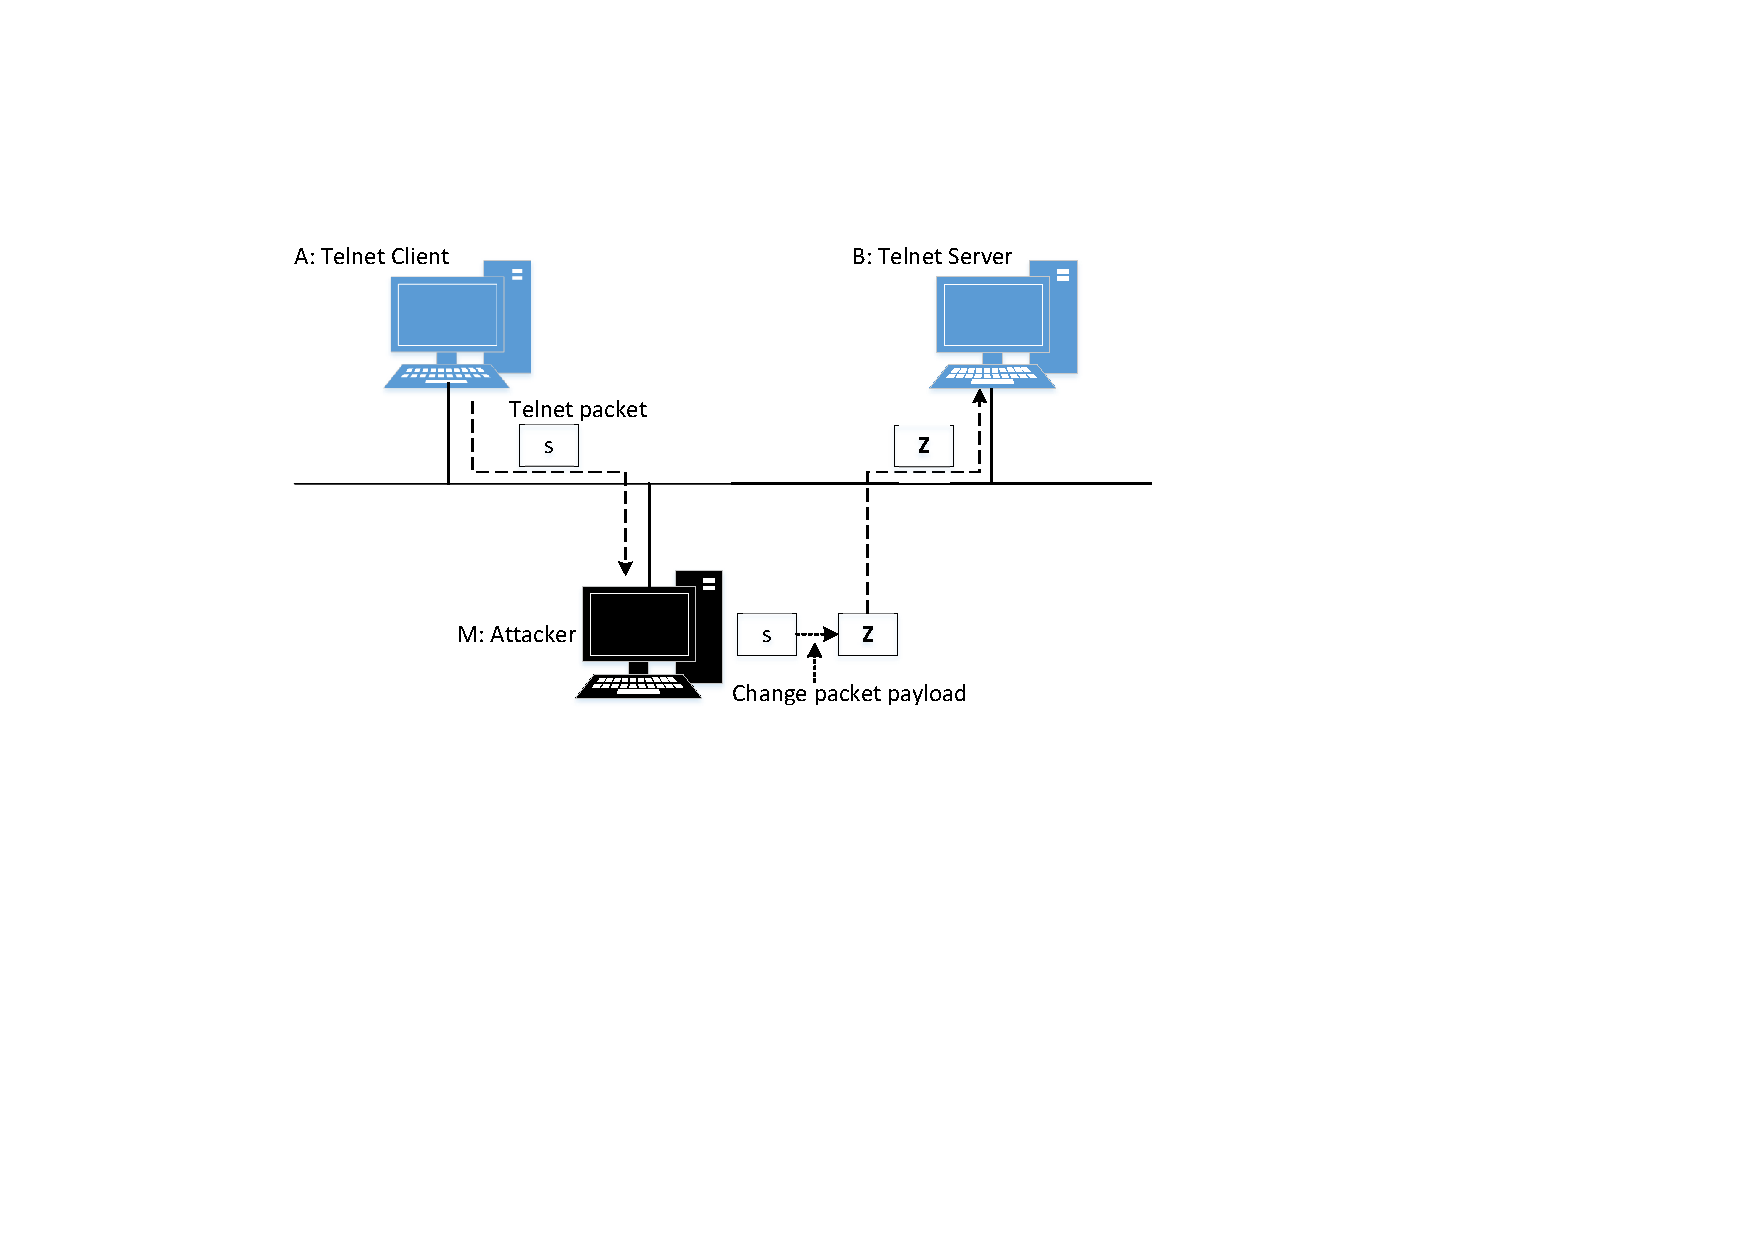
\includegraphics[width=0.8\textwidth]{\arpFigs/telnet_mitm.pdf}
    \caption{Man-In-The-Middle Attack against telnet}
    \label{arp:fig:telnet_mitm}
\end{figure}


\paragraph{Step 1 (Launch the ARP cache poisoning attack).} First, Host M conducts an ARP cache
poisoning attack on both A and B, such that in A's ARP cache, B's IP address maps to M's MAC
address, and in B's ARP cache, A's IP address also maps to M's MAC address. After this step,
packets sent between A and B will all be sent to M. We will use the ARP cache poisoning attack
from Task 1 to achieve this goal. 


\paragraph{Step 2 (Testing).} After the attack is successful, please try to ping each other
between Hosts A and B, and report your observation. Please show Wireshark results in your
report.

\paragraph{Step 3 (Turn on IP forwarding).} Now we turn on the IP forwarding on Host M, so it
will forward the packets between A and B. Please run the following command and repeat Step 2.
Please describe your observation. 

\begin{lstlisting}
$ sudo sysctl net.ipv4.ip_forward=1
\end{lstlisting}

\paragraph{Step 4 (Launch the MITM attack).} We are ready to make changes to the Telnet data
between A and B. Assume that A is the Telnet client and B is the Telnet server. After A has
connected to the Telnet server on B, for every key stroke typed in A's Telnet window, a TCP
packet is generated and sent to B. We would like to intercept the TCP packet, and replace each
typed character with a fixed character (say Z). This way, it does not matter what the user
types on A, Telnet will always display Z.

From the previous steps, we are able to redirect the TCP packets to Host M, but instead of
forwarding them, we would like to replace them with a spoofed packet. We will write a
sniff-and-spoof program to accomplish this goal. In particular, we would like to do the
following: 

\begin{itemize}

\item We first keep the IP forwarding on, so we can successfully create a Telnet connection
between A to B. Once the connection is established, we turn off the IP forwarding using the
following command. Please type something on A's Telnet window, and report your observation: 

\begin{lstlisting}
$ sudo sysctl net.ipv4.ip_forward=0
\end{lstlisting}

\item We run our sniff-and-spoof program on Host M, such that for the captured packets sent
from A to B,  we spoof a packet but with TCP different data. For packets from B to A (Telnet
response), we do not make any change, so the spoofed packet is exactly the same as the original
one. 
\end{itemize} 

To help students get started, we provide a skeleton sniff-and-spoof
program in the following. The program capture all the TCP packets, and 
then for packets from A to B, it makes some changes (the modification
part is not included, because that is part of the task). For packets from
B to A, the program simply forward the original packets. 

\begin{lstlisting}
#!/usr/bin/python3
from scapy.all import *

VM_A_IP = "10.0.2.6"
VM_B_IP = "10.0.2.7"

def spoof_pkt(pkt):
  if pkt[IP].sr == VM_A_IP and pkt[IP].dst == VM_B_IP \
                           and pkt[TCP].payload:

     # Create a new packet based on the captured one.
     # (1) We need to delete the checksum fields in the IP and TCP headers, 
     #     because our modification will make them invalid.
     #     Scapy will recalculate them for us if these fields are missing. 
     # (2) We also delete the original TCP payload.
     newpkt = IP(pkt[IP])
     del(newpkt.chksum)  
     del(newpkt[TCP].chksum) 
     del(newpkt[TCP].payload) 

     #####################################################################
     # Construct the new payload based on the old payload.
     # Students need to implement this part.

     olddata = pkt[TCP].payload.load   # Get the original payload data 
     newdata = olddata  # No change is made in this sample code
     #####################################################################

     # Attach the new data and set the packet out
     send(newpkt/newdata)

  elif pkt[IP].src == VM_B_IP and pkt[IP].dst == VM_A_IP:
     send(pkt[IP]) # Forward the original packet

pkt = sniff(filter='tcp',prn=spoof_pkt)
\end{lstlisting}


It should be noted that the code above captures all the TCP 
packets, including the one generated by the program itself. That is 
undesirable, as it will affect
the performance. Students needs to change the filter, so it does not capture 
its own packets. 


\paragraph{Behavior of Telnet.}
In Telnet, typically, every character we type in the Telnet window triggers
an individual TCP packet, but if you type very fast, some characters may be 
sent together in the same packet. 
That is why in a typical Telnet packet from client to server, 
the payload only contains one character.  The
character sent to the server will be echoed back by the server, 
and the client will then display the
character in its window. Therefore, what we see in the client window is not the direct result
of the typing; whatever we type in the client window takes a round trip before it is displayed.
If the network is disconnected, whatever we typed on the client window will not displayed,
until the network is recovered. Similarly, if attackers change the character to Z during the
round trip, Z will be displayed at the Telnet client window, even though
that is not what you have typed.





% *******************************************
% SECTION
% ******************************************* 
\section{Task 3: MITM Attack on Netcat using ARP Cache Poisoning}

This task is similar to Task 2, except that
Hosts A and B are communicating using \texttt{netcat}, instead of \texttt{telnet}.
Host M wants to intercept their
communication, so it can make changes to the data sent between A and B.
You can use the following commands to establish a \texttt{netcat} TCP
connection between A and B:


\begin{lstlisting}
On Host B (server, IP address is 10.0.2.7), run the following:
$ nc -l 9090

On Host A (client), run the following:
$ nc 10.0.2.7 9090
\end{lstlisting}
 

Once the connection is made, you can type messages on A.
Each line of messages will be put into a TCP packet sent 
to B, which simply displays the message.  
Your task is to replace every occurrence of your first name in the 
message with a sequence of A's. The length of the sequence should be the 
same as that of your first name, or you will mess up the TCP sequence
number, and hence the entire TCP connection. You need to use your real
first name, so we know the work is done by you.  



% *******************************************
% SECTION
% ******************************************* 
\section{Submission}

\seedsubmission


\end{document}



